\documentclass[a4paper,12pt,latin modern roman]{article}
\usepackage{endnotes}
\usepackage{tabularx}
\usepackage{amssymb,amsmath,amsthm,amsfonts}
\fontfamily{latin-modern}
\usepackage{color}
\usepackage[hyphens]{url}
\setlength{\parindent}{0mm}
\setlength{\parskip}{\medskipamount}
\usepackage{graphicx}
\usepackage{amsmath}
\usepackage{endnotes}
%\usepackage{fancyvrb}
\usepackage[section]{placeins}
\usepackage{graphicx}
\usepackage{amssymb,amsmath,amsthm,amsfonts}
\usepackage{float}
%\usepackage{color}
\usepackage[nottoc,numbib]{tocbibind}
\usepackage{url}
\usepackage{lmodern}
\usepackage{verbatim}
\usepackage{enumerate}
\usepackage{abstract}
\usepackage{float}
\usepackage{graphicx}
%\usepackage{hyperref}
\usepackage{algorithm2e}
\usepackage{amsmath}
\usepackage{url}
%\usepackage{lmodern}
\usepackage{graphicx}
\usepackage{fixltx2e}
\usepackage{float}
\linespread{1.25}
\usepackage{url}
\usepackage{graphicx}%<----remove demo in your file
\usepackage{wrapfig}
\usepackage{lscape}
\usepackage{rotating}
\usepackage{epstopdf}
\usepackage[nottoc]{tocbibind}
\newcommand{\superscript}[1]{\ensuremath{^{\textrm{#1}}}}
\usepackage{hyperref}
\hypersetup{
colorlinks=true, %set true if you want colored links
linktoc=all, %set to all if you want both sections and subsections linked
linkcolor=blue, %choose some color if you want links to stand out
citecolor=red 
}
%Gummi|063|=)
\begin{document}
\thispagestyle{empty}
\title{\bf Reinforcement Learning Based Chess}
\maketitle
\centerline{N Puneeth}
\centerline{puneeth.n@iiitb.org}
\vspace{0.2in}
\centerline{Rahul AR}
\centerline{rahul.ar@iiitb.org}
\vspace{0.2in}
\centerline{Sindhu Priyadarshini}
\centerline{sindhu.priyadarshini@iiitb.org}
\vspace{0.5in}
\centerline{\textbf{International Institute of Information Technology, Bangalore}}
\vspace{0.1in}
\vspace{0.1in}
\centerline{\textbf{Machine Learning Project Report}}
\thispagestyle{empty}
\newpage
\thispagestyle{empty}
\begin{center}
\textbf{\large{Abstract}}\\
\par\end{center}
A Reinforcement Learning based Chess engine aims to create a system where we learn the moves from one of the standard chess engines. The program keeps getting better with training. We have chosen Stockfish 4 as our teacher engine which is the most powerful open source chess engine in the world. We have used Artificial Neural Networks with Backpropagation to learn the game.    \\\\\\
\centerline{\textbf{Project URL}: \url {https://github.com/rahular/rStock}  }
\centerline{\textbf{} \url {https://github.com/rahular/rStockTrainer}  }
\vspace{0.5in}
\vfill
\copyright 2013 N Puneeth, Rahul AR, Sindhu Priyadarshini. This material is available under the Creative Commons Attribution-Noncommercial-Share Alike License.\\ See \url{http://creativecommons.org/licenses/by-nc-sa/3.0/} for details.
\newpage
\thispagestyle{empty}
\begin{center}
\textbf{\large{\emph{Acknowledgement}}}
\end{center}
We would like to extend our deepest regards to our advisor, \\\textbf{\emph{Prof. G. Srinivasaraghavan}} for his motivating words and useful suggestions throughout this project. It was a pleasure for us to work under his guidance.\\
We are very grateful to all the people who have helped and supported us during the project. We would also like to extend our gratitude to all the authors whose papers we have referred during the course of our project.
\newpage
\thispagestyle{empty}
\pagenumbering{arabic}
\tableofcontents
\newpage
\thispagestyle{empty}
\listoffigures{}
\newpage
\section{Introduction}
\subsection*{Objective}
The main objective of the project is to develop a chess engine which has to learn from a teacher just as a child would and get better with time.
\subsection*{Motivation}
Reinforcement learning helps us in learning the optimal behavior for processes and tasks which require the selection of sequential actions from a user or an agent. This kind of learning procedure is based on a series of interactions between the agent and its environment. Through repeated interactions with the environment, and the receipt of rewards, the agent learns which actions are associated with the greatest cumulative reward.

The project aims to build a reinforcement learning based chess playing pro-
gram. The aim is to make the program train against other established chess
engines and if necessary, game annotations of some Grandmaster level games. We will
evolve a scheme for the program to gradually play against tougher and
tougher opponents as it plays more and more.
We will define measures to quantify how good a player the program is,
establish that it is actually improving with more and more games played and thus try to emulate the human learning behavior.

\section{Overview}
We are to teach a machine to learn from another machine. In effect we just need to enable a good system (teacher) to pass on its knowledge to another system (learner). This is easier than imparting human knowledge to the computer atleast theoritically since we are to transfer "knowledge" between two similar models of computation.  

\section{Background Study}
The complexity of chess makes it impossible for computers to explore every possible move throughout the whole space of possible moves and pick the best one. Most chess engines therefore focus on a modified brute force strategy to search in the space of the next 'n' possible moves where 'n' is a certain depth. Many pruning processes are used which incorporate intuitive discarding strategies in order to evaluate which is the next best move. Algorithms like alpha-beta pruning and mini-max algorithms seek to find the next best move based on some hardcoded rules. There exists no successful engines which learn and improve over time.

The traditional reinforcement learning strategies have a few key salient features. Firstly, and most importantly all of them try to estimate the value of functions, which becomes a humongous task in case of chess. Secondly, state trajectories of systems are stored and the values are backed up along the actual or possible state trajectories, which again is not a feasible process to mimic the learning behavior of a complex system such as Chess. Thirdly, there is the GPI or the generalized policy iteration, which entails maintaining of two things: A approximate value function and an approximation policy; both of which are continuously improved upon. This again adds to the complexity of learning. 

So we decided that an artificial neural network model will be best suited for teaching as we are training a new engine from scratch. Unlike some newer learning engines which use feature extraction techniques for training, we do not use any such methods so that we can emulate the learning which a real novice, for e.g. a human kid does, i.e. mainly watch and learn from whatever the guardian says is right.  

\section{System Architecture}


\begin{figure}[!ht]
\centering
    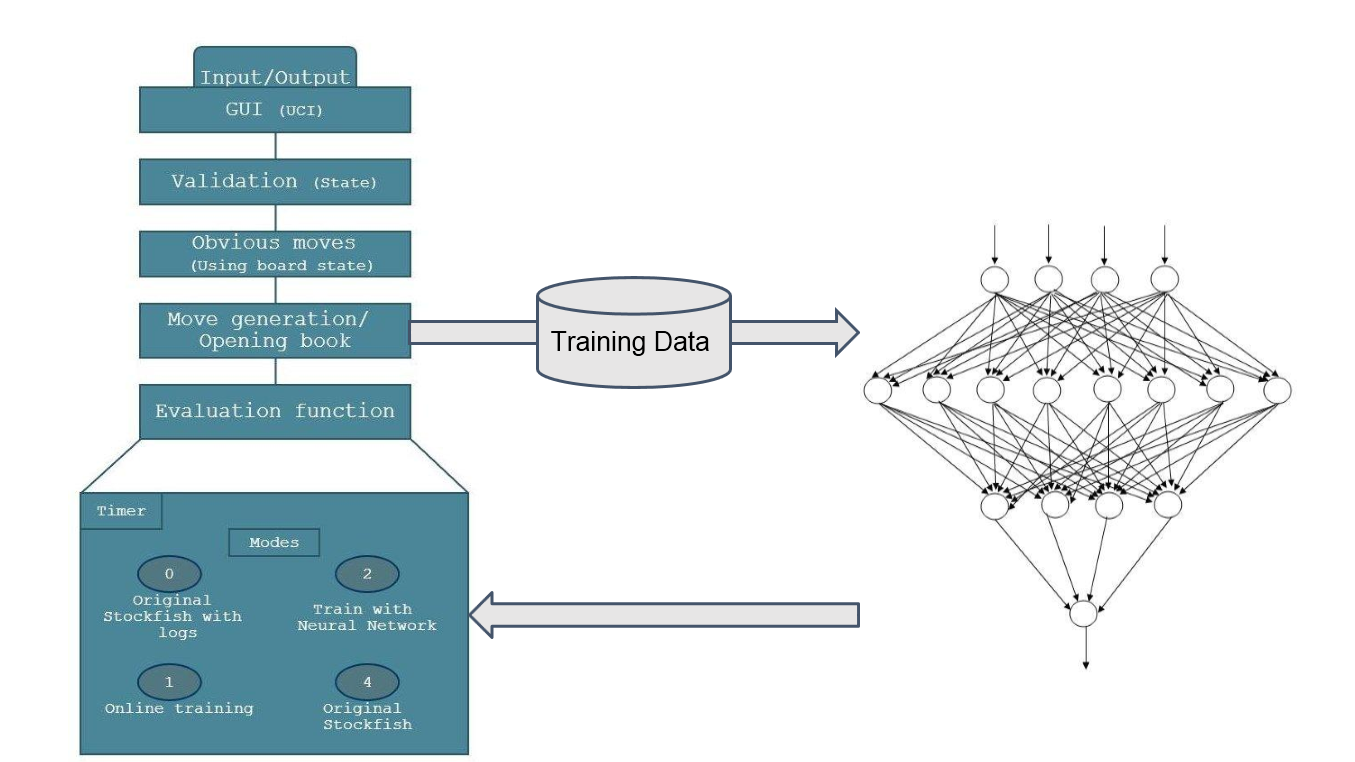
\includegraphics[width=\textwidth,height=\textheight,keepaspectratio]{SysArch.png}%<---angle here
    \caption{System Architecure}

\end{figure}

The architecture has 4 basic parts:


\begin{enumerate}
\item \textbf{Teacher}\\
We have used Stockfish as our teacher engine as it is the most successful and powerful open source chess engine with an ELO rating of 3222 (as of November, 2013). We have used it in conjunction with SCID which is a UCI based GUI for chess play and analysis. We use this engine to create a dataset of board positions (thinking lines) which have been churned out by Stockfish before it makes a move during gameplay. 
\item \textbf{Trainer/Tester}\\
The function of the trainer/tester is to pick up the data which has been generated by the teacher (Stockfish) and train our neural network player on it. This is parallelized to a certain extent so that the training happens faster and no the number of epochs achieved per hour increases.
\item \textbf{Player:}\\
This player is the actual position evaluation function to which we want to teach Chess. The level of learning exhibited by our player depends on the kind of dataset i.e. the thinking lines which it has encountered while training. This is one of the potential problems we face during training i.e if the training data lacks in some quality of gameplay, say defence, the player becomes extremely attacking in nature and tries to maximize the loss of the opponent and neglects its own pieces' safety. 
\item \textbf{User Interface}\\
We have used a fork of SCID, called SCID vs PC. as our UI. SCID which stands of Shane's Chess Information Database, which is a popular chess GUI for Linux and is mainly used for analysis and to study game databases. 
\end{enumerate}


\section{Neural Network}
The Neural Network which we implemented had the following specifications:


\begin{enumerate}
\item \textbf{Input}\\
Input given to the network is an FEN string (converted to binary), along with an evaluation score from Stockfish's original evaluation function which acts as the expected output. 
\item \textbf{Output}\\
Output will be a number between -1 and +1 (later scaled by a factor of 30000). More negative the output, more favorable it is to the black player and vice versa. 
\item \textbf{Input Layer}\\
The Input which we given is basically encoded into 262 bits, 4 bits each for every board sqaure, and 6 more to keep track of the turn, castling options (king/queen side) and en passant. So totally we have 262 input neurons in the Input layer. 
\item \textbf{Hidden Layers}\\
We have experimented with the number of hidden neurons and the number of hidden layers. The number of hidden neurons vary from 128 to 256 and the number of hidden layers vary between 2 to 3. 
\item \textbf{Output Layer}\\
A single neuron acts as the output. 
\item \textbf{Activation Function}\\
We have used a sigmoidal function for activation across all neurons. 
\item \textbf{Learning Rate}\\
We have experimented with learning rates between 0.01 to 0.1 and found 0.05 to be somewhat optimal.
\item \textbf{Momentum}\\
We have set the Momentum to be 0.35 (again based on trial and error)
\item \textbf{Weight Updation:}\\
The weight updation happens according to the backpropagation rule.
\end{enumerate}


\section{Implementation}
\begin{figure}[!ht]
\centering
    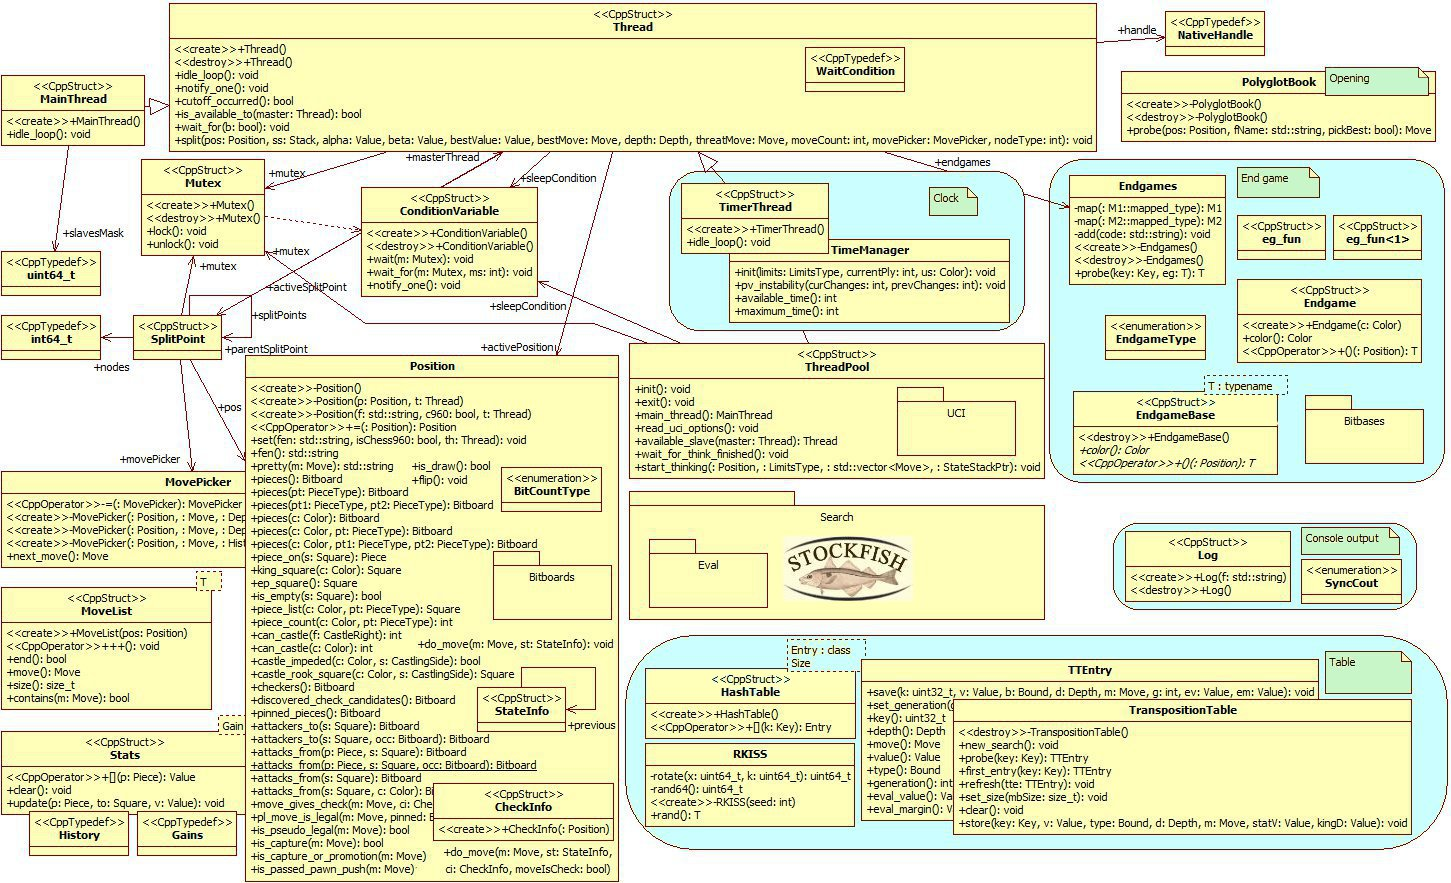
\includegraphics[width=\textwidth,height=\textheight,keepaspectratio]{sf_uml.jpg}%<---angle here
    \caption{StockFish UML diagram}

\end{figure}
We have created a fork to the original UCI Stockfish to incorporate reinforcement learning and neural network into it. 
\\
The Primary programming language which have used to implement our system is C++, and the complete source code with instructions is available at the URL mentioned in the abstract. \\
We have modified the eval and search module to incorporate our neural network into the standard Stockfish engine and created different modes so that we can incorporate both the teacher and the player inside a single system. We have incorporated 4 different modes into Stockfish itself so as to avoid redundancy of code.

\begin{itemize}
\item \textbf{Mode 0}\\
This mode is used to play the default Stockfish engine but with a logging function which writes its thinking lines on to a dump file which acts as the training data for the network. 
\item \textbf{Mode 1}\\
This mode is used to train the neural network in an online manner. The network is trained as and when the teacher thinks i.e the training data is provided to the network during the game itself. This mode is highly time consuming because the teacher generally thinks at a depth of 16 to 20 which means the number of thinking lines is exponential in depth. Therefore this mode is not ideal.
\item \textbf{Mode 2}\\
This mode replaces the original evaluation function of Stockfish with the trained neural network. This means that the learner engine plays without any help from the teacher.
\item \textbf{Mode 3}\\
This mode is the original stockfish engine without any modifications.
\end{itemize}


\section{Testing and Performance}

\begin{itemize}
\item \textbf{Performance}\\
The learning depends on quality of thinking lines.
\item \textbf{Analysis}\\
The ability for complex analysis is weak, since we totally depend on the data which we are exposed to.
\item \textbf{Network-Data-Performance Trade Off:}\\
The three layer network seemed better when compared to a two layer network but when we played them against each other, the two layer performed better which was due to the kind of training data on which they were trained.
\end{itemize}

\section{Conclusion and Future Work}

Neural Networks do not seem ideal for a game like chess. Primary reason being that there are way too many cases to understand, in the order of \begin{math}10^{53}\end{math} to be precise. The computation time it took to train each neural network was also very unreasonable, close to 24 hours on a 4-core i5 machine (after parallelization). We may be able to increase this throughput by integrating end-game books and so on, to make the learning more effective. We can also try to ensemble multiple algorithms to boost the performance. 

\pagebreak
\begin{thebibliography}{}
\bibitem{G} Mannen, Henk, and M. A. Wiering. "Learning to play Chess using TD (lambda)-learning with database games." (2004): 72-79.
1998.
\bibitem{S} S.Thrun. "Learning to Play the Game of Chess".NIPS 7. MIT Press. 1995.
\bibitem{SF} Stocfish. A Powerful Open source Chess Engine. URL: http://stockfishchess.org/.
\bibitem{UI} SCID. Shane's Chess Information Database. A Chess Toolkit.  URL:http://scid.sourceforge.net/
\bibitem{UI} SCID vs PC. A Usability and bug fix fork of SCID. URL:http://scidvspc.sourceforge.net/


\end{thebibliography}
\end{document}
